\documentclass[a4paper,12pt]{article}
\usepackage{amsmath,amssymb,amsfonts,amsthm}
\usepackage{tikz}
\usepackage[utf8x]{inputenc}
\usepackage[T2A]{fontenc} 
\usepackage[russian]{babel}
\usepackage{cmap} 
\usepackage{ gensymb }
% Так ссылки в PDF будут активны
\usepackage[unicode]{hyperref}
\usepackage{ textcomp }
\usepackage{indentfirst}
\usepackage[version=3]{mhchem}

% вы сможете вставлять картинки командой \includegraphics[width=0.7\textwidth]{ИМЯ ФАЙЛА}
% получается подключать, как минимум, файлы .pdf, .jpg, .png.
\usepackage{graphicx}
% Если вы хотите явно указать поля:
\usepackage[margin=1in]{geometry}
% Или если вы хотите задать поля менее явно (чем больше DIV, тем больше места под текст):
% \usepackage[DIV=10]{typearea}

\usepackage{fancyhdr}

\newcommand{\bbR}{\mathbb R}%теперь вместо длинной команды \mathbb R (множество вещественных чисел) можно писать короткую запись \bbR. Вместо \bbR вы можете вписать любую строчку букв, которая начинается с '\'.
\newcommand{\eps}{\varepsilon}
\newcommand{\bbN}{\mathbb N}
\newcommand{\dif}{\mathrm{d}}

\newtheorem{Def}{Определение}


\pagestyle{fancy}
\makeatletter % сделать "@" "буквой", а не "спецсимволом" - можно использовать "служебные" команды, содержащие @ в названии
\fancyhead[L]{\footnotesize Квантовая физика}%Это будет написано вверху страницы слева
\fancyhead[R]{\footnotesize ФМХФ МФТИ}
\fancyfoot[L]{\footnotesize \@author}%имя автора будет написано внизу страницы слева
\fancyfoot[R]{\thepage}%номер страницы —- внизу справа
\fancyfoot[C]{}%по центру внизу страницы пусто

\renewcommand{\maketitle}{%
	\noindent{\bfseries\scshape\large\@title\ \mdseries\upshape}\par
	\noindent {\large\itshape\@author}
	\vskip 2ex}
\makeatother
\def\dd#1#2{\frac{\partial#1}{\partial#2}}


\title{10.1 \\ Электронный парамагнитный резонанс}
\author{Егор Берсенев} 
\date{16 февраля 2017 г.}

\begin{document}
	
	\maketitle
	\section{Теоретическое введение}
		Энергетический уровень электрона в присутствии магнитного поля $B$ расщепляется на два подуровня, расстояние между которыми равно:
		\begin{equation}
		    \Delta E = E_2 - E_1 = 2\mu B
		\end{equation}
		Между этими двумя уровнями возможны переходы. Они могут возбуждаться внешним высокочастотным магнитным полем подходящих характеристик.
		Резонансное значение частоты определяется из очевидного соотношения:
		\begin{equation}
		    \hbar\omega_0 = \Delta E =2\mu B
		\end{equation}
	    При переходе с нижнего на верхний уровень квант энергии поглощается, а при обратном переходе излучается квант той же частоты. Возбуждение электронных резонансных переходов электромагнитным полем с частотой $\omega_0$ носит название <<электронного парамагнитного резонанса>>
	    Сигнал ЭПР наблюдается только на неспаренных электронах образца. В работе используется образец свободного радикала ДФПГ.
	    \begin{figure}[h!]
			\centering
			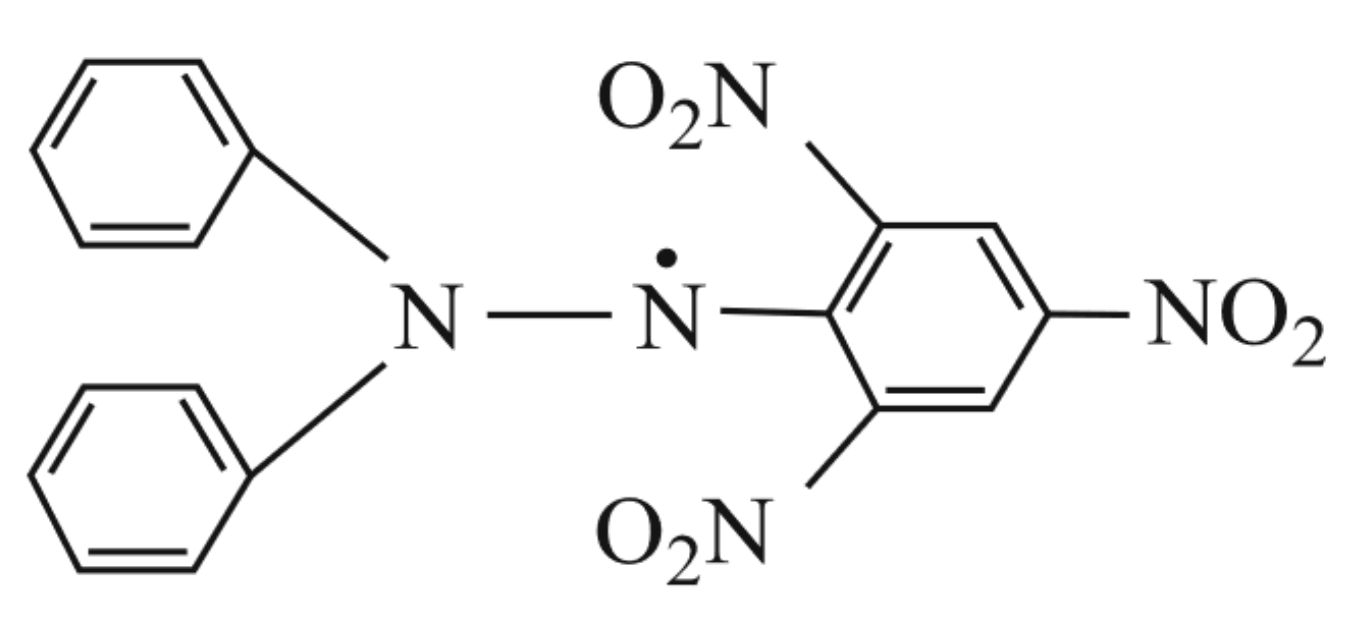
\includegraphics[width=0.5\linewidth]{dfpg}
			\caption{Дифенилпикрилгидразил}
		\end{figure}
    Рассмотрим основные процессы, влияющие на ширину линии ЭПР. В отсутсвие высокочастотного поля заселенность верхнего и нижнего уровней $N_u$ и $N_d$ определяется температурой и описывается формулой Больцмана.
    \begin{equation}
        \frac{N_u}{N_d} = exp\left(-\frac{\Delta E}{kT}\right)
    \end{equation}
    В присутствии резонансного поля между уровнями возникают индуцированные переходы, ведущие к тому, что заселенность верхнего уровня растет, а нижнего падает. Этот процесс ведет к нарушению соотношения Больцмана. Восстановление теплового равновесия происходит двумя способами: спин-спиновой и спин-решеточной релаксацией.
    Отличить их друг от друга можно по температурной зависимости: спин-решеточное взаимодействие быстро возрастает с температурой(числом фононов), спин-спиновое от температуры практически не зависит.
    Согласно соотношению неопределенностей:
    \begin{equation}
        \Delta\omega\tau \simeq 1
    \end{equation}
	
	\section{Описание эксперимента}
        В работе требуется получить ЭПР сигнал на ДФПГ. Известно, что связь между магнитным моментом электрона и его механическим моментом выражается через гиромагнитное соотношение:
        \begin{equation}
            \bf{\mu} = \gamma\bf{M}
        \end{equation}
        Если магнитный момент выражается в магнетонах Бора, а механический в единицах $\hbar$, то связь выражается через фактор Ланде:
        \begin{equation}
            \frac{\bf{\mu}}{\mu_B} = \frac{g\bf{M}}{\hbar}
        \end{equation}
        Эта формула справедлива и для проекций. Можно выразить $g$-фактор через определяемые экспериментально величины:
        \begin{equation}
            g = \frac{\hbar\omega_0}{\mu_B B}
        \end{equation}
        Схема спектроскопа приведена на рисунке:
        \begin{figure}[h!]
			\centering
			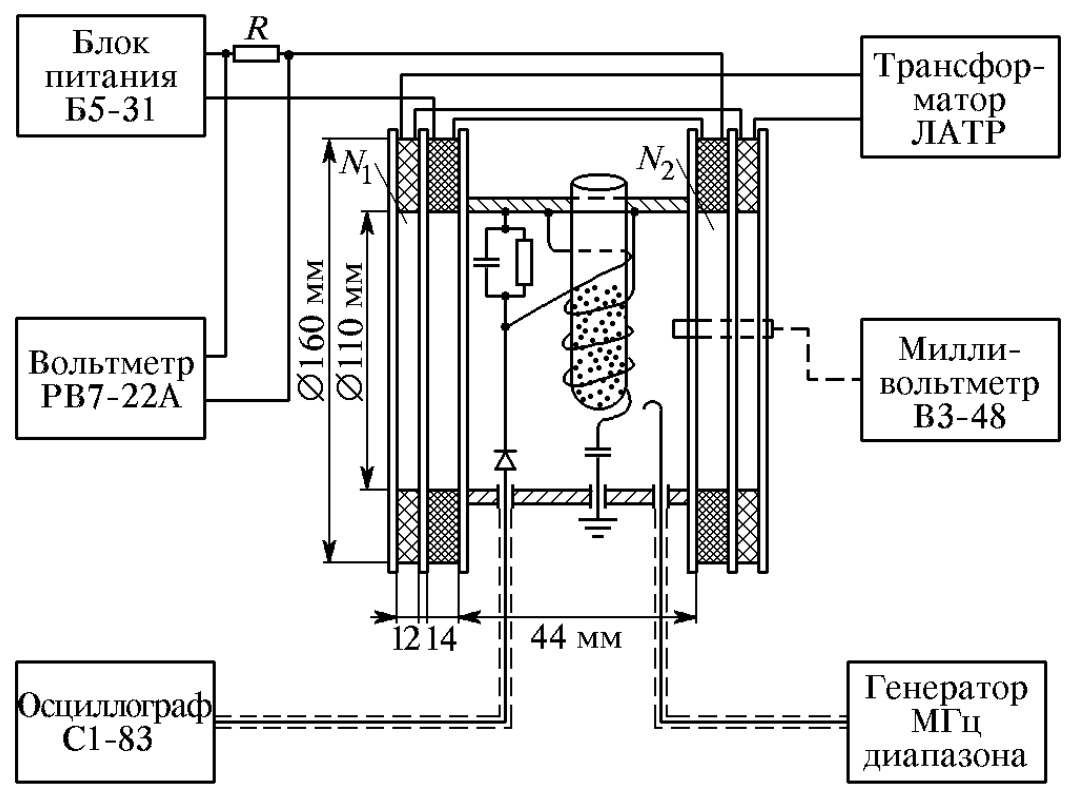
\includegraphics[width=0.5\linewidth]{exp}
			\caption{Схема установки}
		\end{figure}        
		
		Параметры установки: $N_1 = 1500, d_1 = 0.23\,cm, N_2 = 4500, d_2=0.29\,cm$
    \section{Экспериментальные данные}
    Настроим генератор на резонансную частоту колебательного контура, определили значение частоты при максимальном и половинных значениях амплитуды выведенного на осциллограф сигнала:
	
	$f_{0} = 126.76 \, \text{МГц}$
	
	$f_{h} = 126.97 \, \text{МГц}$
	
	$f_{l} = 126.49 \, \text{МГц}$
	
	Рассчитаем добротность
    
    $$ Q = \frac{f}{\Delta f} = \frac{126.76}{0.48} = 264.1 $$
    
    Теперь настроим установку на наблюдение резонансного сигнала. Резонансное поглощение возникает при совпадении в некоторые моменты времени поля $B(t)$ с полем резонансного поглощения на частоте колебательного контура $B_0=\frac{\mathrm{h}f_0}{g\mu_B}$
    
    \begin{figure}[h!]
			\begin{center}
				\begin{minipage}{0.49\linewidth}
					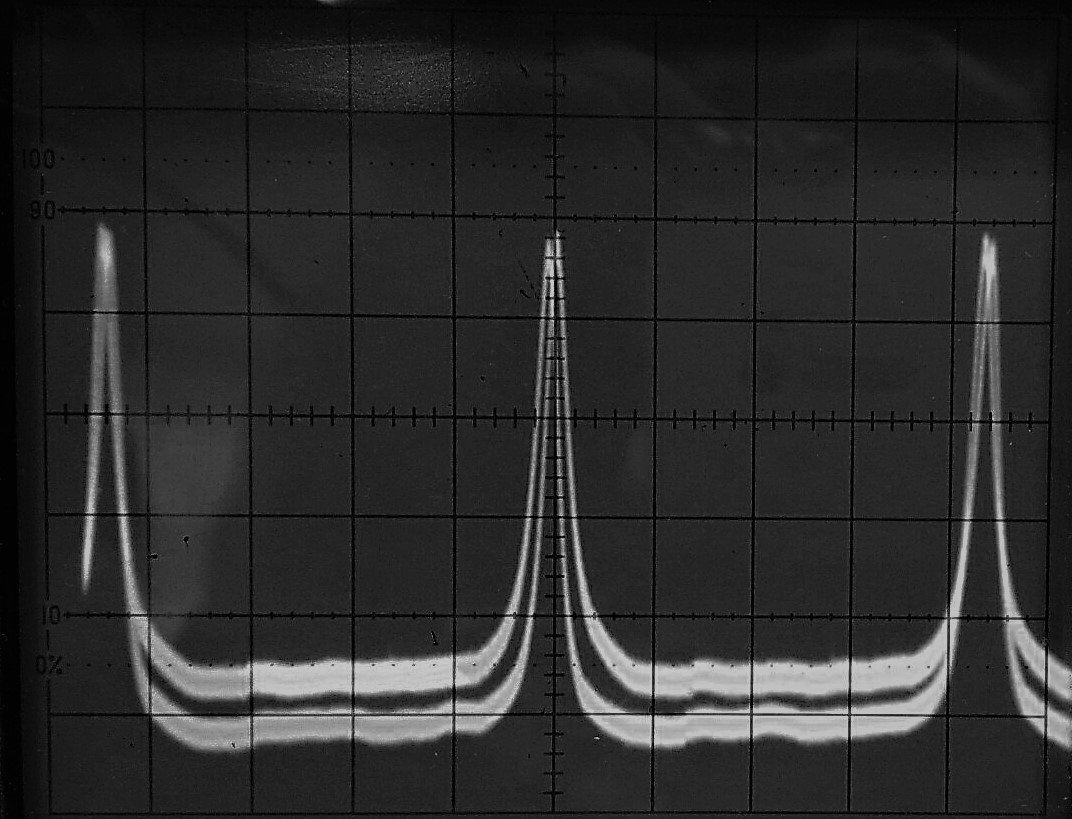
\includegraphics[width=\linewidth]{oscilloscope.jpg}
					\caption{Резонансное поглощение}
				\end{minipage}
				\hfill
				\begin{minipage}{0.49\linewidth}
					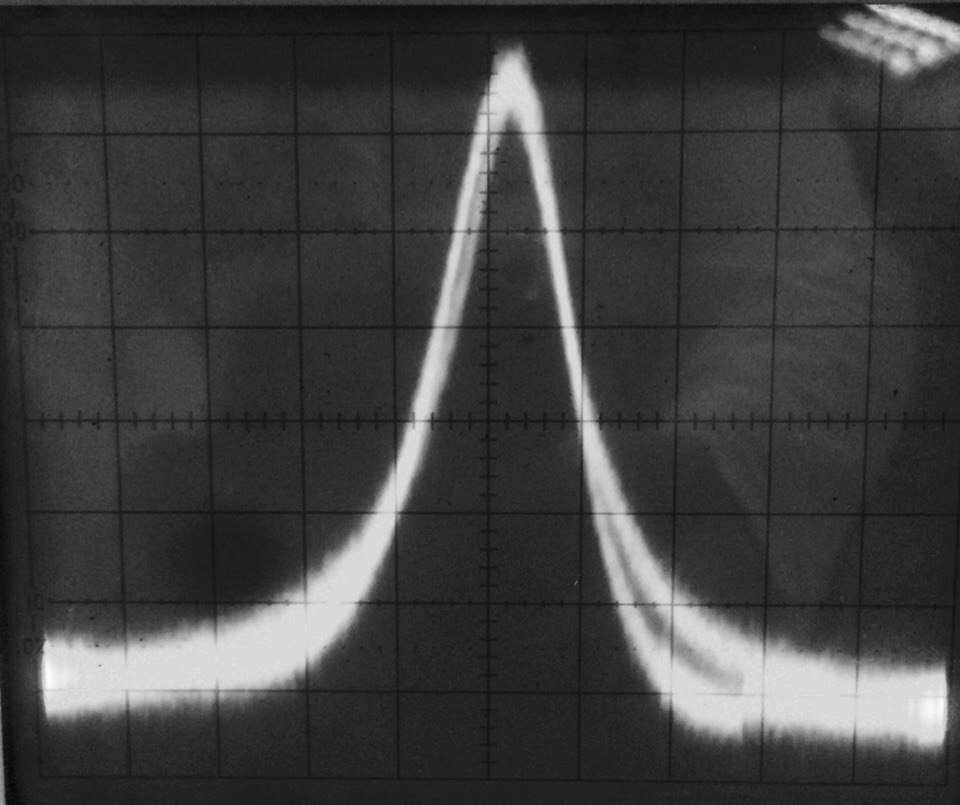
\includegraphics[width=\linewidth]{second.jpg}
					\caption{Точно настроенный пик}
				\end{minipage}
			\end{center}
		\end{figure}

    
    
    Переменное поле модуляционных катушек наводит в пробной катушке ЭДС индукции,
по которой можно определить величину поля. 
Зная параметры катушки $N_{проб} = 45$, $d = 15.2 \pm 0.1 \; мм$ и ЭДС, определим величину модулирующего поля:

\begin{equation}
B_{мод} = \sqrt{2} \frac{2\varepsilon_i}{\pi^2 d^2N_{проб} \nu} = \sqrt{2} \frac{2 \cdot 2.51 \cdot 10^{-3}\, \text{В}}{\pi^2 \cdot 14.5^2 \cdot 10^{-6} \, \text{м} \cdot 45 \cdot 50\, \text{Гц}}  = 1.52 \cdot 10^{-3} \,\text{Тл} = 1.52 \, \text{мТл}
\end{equation}

тогда для полуширины на полувысоте линии резонансного поглощения (в единицах поля) получим

\begin{equation}
\Delta B  = \frac{A_{1/2}}{A_{\text{полн}}} В_{\text{мод}} = \frac{1}{10.4}\cdot 1.52 = 0.146 \,\text{мТл}  
\end{equation}

Определяем g-фактор. Для этого подаем в основные катушки переменный ток 
), а ЭДС индукции измеряем при помощи пробной катушки. Строим каллиб-
ровочный график:

\begin{figure}
    \centering
    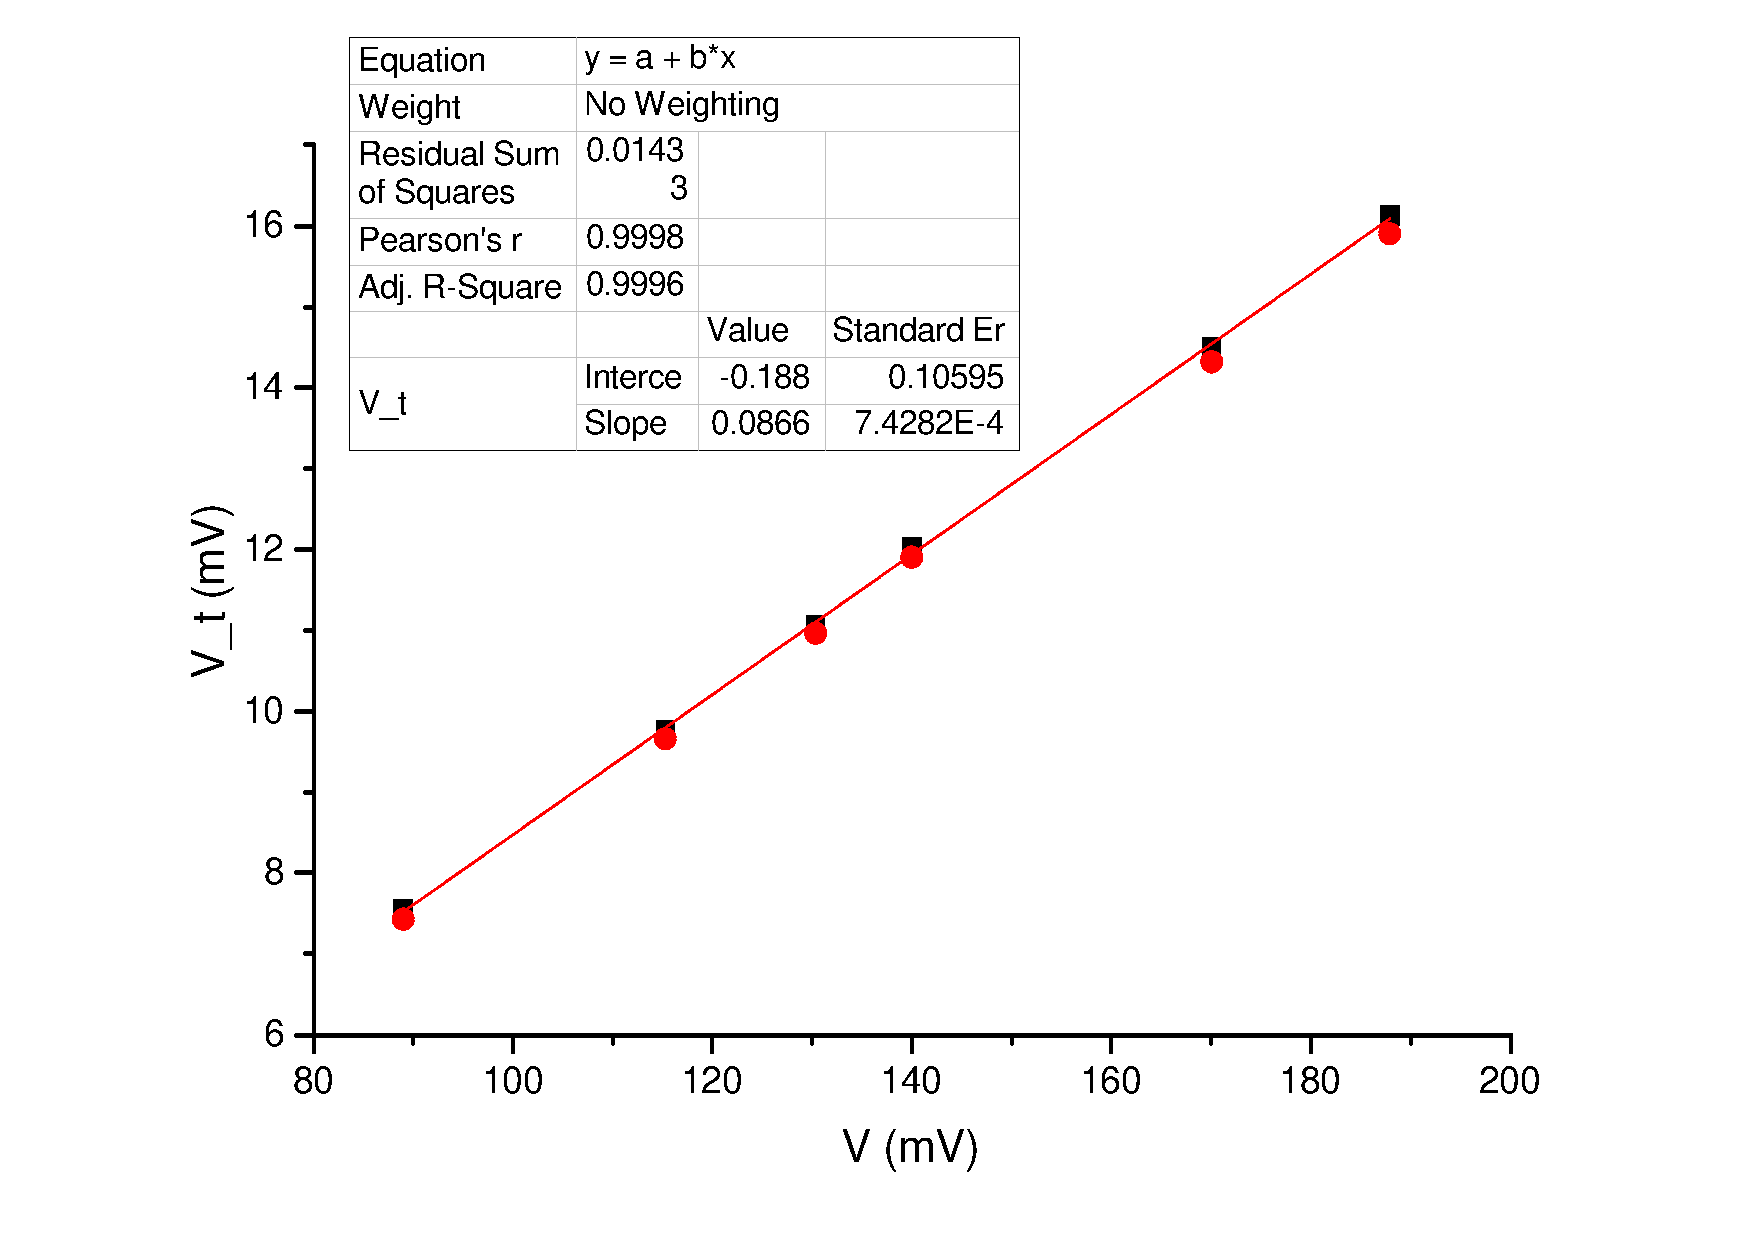
\includegraphics[width = 0.8\linewidth]{cal}
    \caption{ Зависимость ЭДC индукции в пробной катушке от падения напряжения в цепи основных катушек}
    \label{fig:my_label}
\end{figure}
    
    При $V = 122.84\,\mathrm{mV}$ получаем $V_t = 10.45\pm0.08$. Тогда
    \begin{equation}
        B_0 = \frac{V_t}{NS\omega} = 7.03\pm 0.45\,\mathrm{mT}
    \end{equation}
    Отсюда получаем g-фактор равный $g = 1.9\pm0.2$. Вроде сошлось.
    
    
    Построим график зависимости резонасной частоты от тока в цепи основных катушек для проверки линейности расщепления уровней.
    
    \begin{figure}
        \centering
        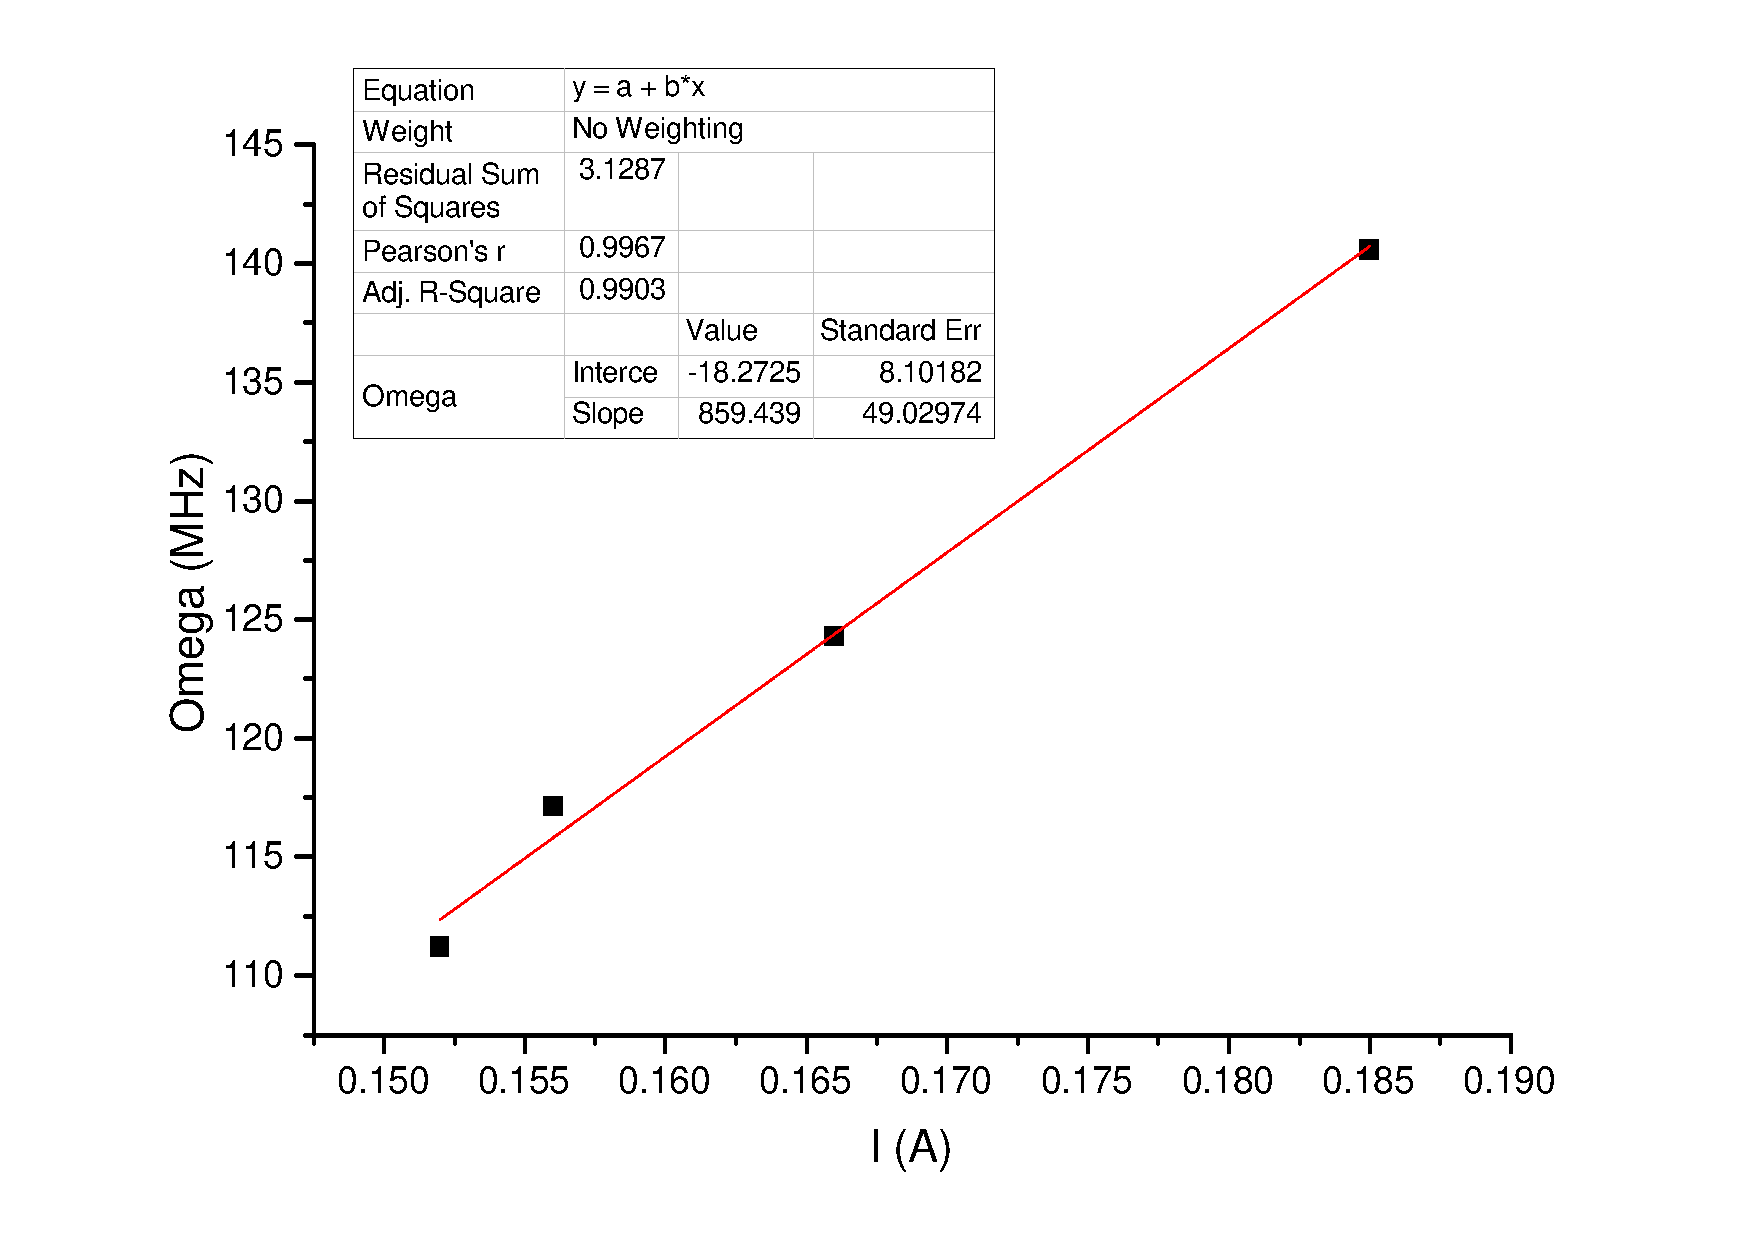
\includegraphics[width = 0.8\linewidth]{lin.pdf}
        \caption{Зависимость резонансной частоты от тока}
    \end{figure}
    
    График, как видно, линейный.
    
    \section{Вывод и обсуждение результатов}
        Рассчитали $g-$фактор, пусть и за месяц, но рассчитали, кроме того было обнаружено, что зеемановской расщепление линейно по полю.
    
\end{document}


